\chapter{Élasticité linéaire} \label{chap:Ch05}
\section{Description du comportement élastique} \label{sec:Ch05-1}
Le modèle de comportement le plus simple est le modèle élastique.
Pour des matériaux ayant un comportement élastoplastique ou viscoplastique, ce modèle convient parfaitement, pourvu que l'on ne dépasse pas le seuil de plasticité.
Pour des matériaux ayant un comportement de type viscoélastique, la transformation de Laplace permet de se ramener à un comportement élastique.
Même pour des matériaux ayant un comportement plus complexe, un calcul élastique peut fournir des résultats intéressants, par exemple pour le calcul des fondations en Mécanique des Sols.
Enfin, la résolution numérique d'un problème de Mécanique des Solides, avec une loi de comportement quelconque, s'effectue presque toujours par résolution d'une suite de problèmes élastiques.
Il est donc naturel, dans un cours de Mécanique des Solides, de réserver une place importante à ce modèle de comportement.

\subsection{Le tenseur d'élasticité} \label{ssec:Ch05-1.1}
Le comportement élastique est caractérisé par une relation linéaire entre contraintes et déformations.
Dans le cadre de l'élasticité tridimensionelle, cette relation s'écrit
\begin{equation}
    \begin{cases}
        \sigma_{ij} = A_{ijkh} \varepsilon_{kh}, & \varepsilon_{ij} = \Lambda_{ijkh} \sigma_{kh} \\
        \tens{\sigma} = A \left[ \tens{\varepsilon} \right], & \tens{\varepsilon} = \Lambda \left[ \tens{\sigma} \right]
    \end{cases}
    \label{eq:Ch05-001}
\end{equation}
où $A_{ijkh}$ et $\Lambda_{ijkh}$ sont les composantes de deux applications $A$ et $\Lambda$, inverses l'une de l'autre, de l'espace des tenseurs symétriques dans lui-même.
Ce sont les tenseurs d'élasticité.
Souvent $A$ est appelé tenseur de rigidité et $\Lambda$ tenseur de complaisance.
Compte-tenu de la symétrie des tenseurs des contraintes et des déformations, on doit avoir, par exemple pour $A$,
\begin{equation}
    A_{ijkh} = A_{jikh} \quad A_{ijkh} = A_{ijhk}
    \label{eq:Ch05-002}
\end{equation}

Nous ferons de plus sur ces applications les deux hypothèses suivantes
\begin{description}
    \item[Hypothèse thermodynamique.] Le tenseur d'élasticité est symétrique
        \begin{equation}
            A_{ijkh} = A_{khij}
            \label{eq:Ch05-003}
        \end{equation}
    \item[Hypothèse de stabilité.] Le tenseur d'élasticité est défini positif
        \begin{equation}
            A_{ijkh} \varepsilon_{ij} \varepsilon_{kh} \geq \alpha \varepsilon_{ij} \varepsilon_{ij}, \quad \alpha > 0
            \label{eq:Ch05-004}
        \end{equation}
\end{description}

La première hypothèse est à peu près invérifiable, mais elle conduit à une théorie bien plus agréable et satisfaisante.
La seconde a une signification tout à fait claire, que nous verrons plus loin.
Compte-tenu des relations de symétrie \eqref{eq:Ch05-002} et \eqref{eq:Ch05-003}, on constate que le tenseur d'élasticité fait apparaître 21 coefficients.
On peut le représenter par une matrice $6\times6$ symétrique
\begin{equation}
    \begin{bmatrix}
        \sigma_{11}\\
        \sigma_{22}\\
        \sigma_{33}\\
        \sigma_{23}\\
        \sigma_{31}\\
        \sigma_{12}
    \end{bmatrix}
    =
    \begin{bmatrix}
        C_{11} & C_{11} & C_{13} & C_{14} & C_{15} & C_{16} \\
        C_{12} & C_{22} & C_{23} & C_{24} & C_{25} & C_{26} \\
        C_{13} & C_{23} & C_{33} & C_{34} & C_{35} & C_{36} \\
        C_{14} & C_{24} & C_{34} & C_{44} & C_{45} & C_{46} \\
        C_{15} & C_{25} & C_{35} & C_{45} & C_{55} & C_{56} \\
        C_{16} & C_{26} & C_{36} & C_{46} & C_{56} & C_{66}
    \end{bmatrix}
    \begin{bmatrix}
        \varepsilon_{11}\\
        \varepsilon_{22}\\
        \varepsilon_{33}\\
        \varepsilon_{23}\\
        \varepsilon_{31}\\
        \varepsilon_{12}
    \end{bmatrix}
    \label{eq:Ch05-005}
\end{equation}

On peut aussi obtenir le comportement élastique par une approche thermodynamique: un matériau élastique est un matériau sans dissipation, c'est à dire un matériau dans lequel toutes les évolutions sont réversibles.
En se plaçant d'un point de vue purement mécanique (on verra comment prendre en compte les variables thermiques au chapitre~\ref{chap:Ch11}), l'équation~\eqref{eq:Ch01-059} donne, puisque la dissipation $\varphi$ est nulle, la relation
\begin{equation}
    \rho \frac{\ud u}{\ud t} = \sigma_{ij} \frac{\ud \varepsilon_{ij}}{\ud t}
    \label{eq:Ch05-006}
\end{equation}
(en petites déformations, $D_{ij} = \ud \varepsilon_{ij} / \ud t$).
Ceci incite à prendre l'énergie interne $u$ fonction des déformations
\begin{equation}
    \rho u = w \left( \tens{\varepsilon} \right)
    \label{eq:Ch05-007}
\end{equation}
où $w$ est le «~potentiel élastique~».
En dérivant \eqref{eq:Ch05-007} et en identifiant avec \eqref{eq:Ch05-006} on obtient
\begin{equation}
    \sigma_{ij} = \frac{\partial w}{\partial \varepsilon_{ij}}
    \label{eq:Ch05-008}
\end{equation}
Les déformations étant petites, on peut développer $w$ en série de Taylor
\begin{equation}
    w \left( \varepsilon_{ij} \right) = w_0 + \cancel{a_{ij} \varepsilon_{ij}} + \frac{1}{2} A_{ijkh} \varepsilon_{ij}\varepsilon_{kh}
    \label{eq:Ch05-009}
\end{equation}
où $a_{ij}$ est symétrique et où $A_{ijkh}$ vérifie les conditions de symétrie \eqref{eq:Ch05-002} et \eqref{eq:Ch05-003} qui, dans cette approche, sont automatiquement vérifiées.
En reportant dans \eqref{eq:Ch05-008} il vient
\begin{displaymath}
    \sigma_{ij} = \cancel{a_{ij}} + A_{ijkh} \varepsilon_{kh}
\end{displaymath}
qui montre que $a_{ij}$ est nul puisque la configuration de référence est supposée libre de contrainte.
On obtient donc \eqref{eq:Ch05-001}, mais avec cette approche l'hypothèse thermodynamique \eqref{eq:Ch05-003} est automatiquement vérifiée, tandis que l'hypothèse de stabilité \eqref{eq:Ch05-004} exprime le fait que l'énergie interne du matériau atteint son minimum dans l'état de référence.
C'est donc bien une hypothèse de stabilité.
En d'autres termes, il faut fournir un travail positif pour déformer le matériau à partir de son état naturel.

Nous introduisons également $\mathop{w}^{*}\left( \tens{\sigma} \right)$, transformée de Legendre de $w$
\begin{equation}
    \mathop{w}^{*}\left( \tens{\sigma} \right) = \sigma_{ij} \varepsilon_{ij} - w \left( \tens{\varepsilon} \right)
    \label{eq:Ch05-010}
\end{equation}
qui permet d'écrire
\begin{equation}
    \varepsilon_{ij} = \frac{\partial \mathop{w}^*}{\partial \sigma_{ij}}
    \label{eq:Ch05-011}
\end{equation}
Finalement, en prenant $w_0=0$, on peut réécrire la loi de comportement élastique \eqref{eq:Ch05-001} sous la forme
\begin{equation}
    \begin{aligned}
        & w = \frac{1}{2} A_{ijkh} \varepsilon_{ij} \varepsilon_{kh} = \mathop{w}^* = \frac{1}{2} \Lambda_{ijkh} \sigma_{ij} \sigma_{kh} \\
        & \sigma_{ij} \frac{\partial w}{\partial \varepsilon_{ij}} = A_{ijkh} \varepsilon_{kh} \\
        & \varepsilon_{ij} = \frac{\partial \mathop{w}^*}{\partial \sigma_{ij}} = \Lambda_{ijkh} \sigma_{kh}
    \end{aligned}
    \label{eq:Ch05-012}
\end{equation}

\subsection{Isotropie et anisotropie} \label{ssec:Ch05-1.2}
Le tenseur d'élasticité, qui caractérise complètement les propriétés élastiques du matériau, dépend, dans le cas le plus général, de 21 coefficients.
Fort heureusernent, on peut restreindre ce nombre en utilisant les symétries du matériau, c'est à dire les propriétés d'isotropie ou d'anisotropie.
Lors d'un changement de repère, les matrices $\sigma_{ij}$ et $\varepsilon_{ij}$ représentatives des tenseurs des contraintes et de déformations se transforment par \eqref{eq:Ch02-007} et \eqref{eq:Ch03-012}.
Les tenseurs d'élasticité $A$ et $\Lambda$ se transforment donc par
\begin{equation}
    A_{ijkh}' = Q_{im} Q_{jn} Q_{kp} Q_{hq} A_{mnpq}
    \label{eq:Ch05-013}
\end{equation}
Les composantes $A_{ijkh}$ du tenseur d'élasticité, ou la matrice d'élasticité \eqref{eq:Ch05-005} dépendent donc du repère choisi.
Les propriétés de symétrie matérielle caractérisent les transformations qui laissent invariantes ces composantes.

On dira qu'un matériau est isotrope si toutes ses directions sont équivalentes, c'est à dire si la matrice d'élasticité \eqref{eq:Ch05-005} est indépendante du repère choisi.
On doit donc avoir, pour tout $A_{ij}$ orthogonal,
\begin{equation}
    A_{ijkh} = Q_{im} Q_{jn} Q_{kp} Q_{kq} A_{mnpq}
    \label{eq:Ch05-014}
\end{equation}
Si, au contraire, il existe des directions privilégiées, le matériau sera dit anisotrope, et la matrice d'élasticité dépendra du repère choisi.
Il conviendra de choisir au mieux ce repère.

Pour caractériser plus précisément l'anisotropie, nous introduisons le groupe d'isotropie $\mathcal{G}$: groupe des transformations orthogonales laissant invariantes les composantes du tenseur d'élasticité.
Si l'on a choisi un repère, $\mathcal{G}$ est le groupe des matrices orthogonales vérifiant \eqref{eq:Ch05-014}.
Il est clair que $\mathcal{G}$ est un sous-groupe du groupe orthogonal.
Si $\mathcal{G}$ est le groupe orthogonal tout entier, alors le matériau est isotrope, sinon le matériau est anisotrope, et l'anisotropie est caractérisée par $\mathcal{G}$.

L'origine physique de l'anisotropie peut être liée soit à la structure du matériau, soit à son mode de formation. 

\paragraph{Anisotropie de structure}
\begin{itemize}
    \item monicristaux métalliques.
        Le groupe d'isotropie est alors le groupe cristallographique.
        Il est à noter que pour les matériaux métalliques polycristallins, habituellement considérés comme isotropes, cette isotropie est de nature statistique; le polycristal est en effet formé de la juxtaposition d'un grand nombre de grains monocristallins, donc anisotropes.
        L'isotropie globale du polycristal résulte donc du caractère aléatoire de la répartition des orientations cristallographiques de chacun des grains.
    \item matériaux composites renforcés par fibres unidirectionnelles ou multi directionnelles -- matériaux composites stratifiés.
        Ces matériaux, de développement relativement récent, permettt d'obtenir des performances très élevées.
    \item matériaux fibreux naturels comme le bois.
\end{itemize}

\paragraph{Anisotropie de formation} pour des matériaux initialement isotropes, mais qui ont été rendus anisotropes par les traitements subis
\begin{itemize}
    \item produits métalliques semi-finis obtenus par forgeage: tôles minces obtenues par laminage et qui présentent trois directions privilégiées (direction de laminage, direction transversale et épaisseur), barres obtenues par filage et qui ont une direction privilégiée.
    \item roches ou sols de nature sédimentaire ou qUl ont subi d'importants 
tassements géologiques.
\end{itemize}

On voit donc que les manifestations de l'anisotropie sont aussi nombreuses que variées.
Nous avons présenté le concept dans le cadre de l'élasticité linéaire, mais le problème se pose pour tout comportement.
Il s'agit néanmoins d'une question difficile et encore imparfaitement comprise. 

\subsection{Élasticité anisotrope} \label{ssec:Ch05-1.3}
Les propriétés de symétrie, décrites par le groupe d'isotropie $\mathcal{G}$, permettent de réduire le nombre des coefficients d'élasticité.
Nous allons envisager quelques cas particuliers correspondant aux types d'anisotropie que l'on rencontre le plus fréquemment en mécanique. 
\subsubsection{Orthotropie}
Il existe trois directions privilégiées mutuellement orthogona1es, et le groupe d'isotropie est formé des symétries laissant invariantes chacune de ces trois directions (non orientées), c'est à dire des symétries par rapport aux axes correspondants.
Si nous choisissons le repère formé par ces trois directions, alors le groupe d'isotropie $\mathcal{G}$ est formé des 4 matrices 
\begin{equation}
    \begin{bmatrix}
        1 & 0 & 0 \\
        0 & 1 & 0 \\
        0 & 0 & 1
    \end{bmatrix}
    \quad
    \begin{bmatrix}
        1 & 0 & 0 \\
        0 & -1 & 0 \\
        0 & 0 & -1
    \end{bmatrix}
    \quad
    \begin{bmatrix}
        -1 & 0 & 0 \\
        0 & 1 & 0 \\
        0 & 0 & -1
    \end{bmatrix}
    \quad
    \begin{bmatrix}
        -1 & 0 & 0 \\
        0 & -1 & 0 \\
        0 & 0 & 1
    \end{bmatrix}
    \label{eq:Ch05-015}
\end{equation}
En écrivant \eqref{eq:Ch05-014} pour ces matrices, on obtient directement la nullité des coefficients $A_{1112}$, $A_{1113}$, $A_{1123}$, $A_{1213}$, etc., et la matrice d'élasticité a la forme suivante 
\begin{equation}
    \begin{bmatrix}
        \sigma_{11}\\
        \sigma_{22}\\
        \sigma_{33}\\
        \sigma_{23}\\
        \sigma_{31}\\
        \sigma_{12}
    \end{bmatrix}
    =
    \begin{bmatrix}
        A_{1} & B_{12} & B_{13} & 0 & 0 & 0 \\
        B_{12} & A_{1} & B_{23} & 0 & 0 & 0 \\
        B_{13} & B_{23} & A_1 & 0 & 0 & 0 \\
        0 & 0 & 0 & C_{4} & 0 & 0 \\
        0 & 0 & 0 & 0 & C_{5} & 0 \\
        0 & 0 & 0 & 0 & 0 & C_{6}
    \end{bmatrix}
    \begin{bmatrix}
        \varepsilon_{11}\\
        \varepsilon_{22}\\
        \varepsilon_{33}\\
        \varepsilon_{23}\\
        \varepsilon_{31}\\
        \varepsilon_{12}
    \end{bmatrix}
    \label{eq:Ch05-016}
\end{equation}
Pour un matériau orthotrope, la matrice élastique ne fait plus intervenir que 9 coefficients.
La matrice d'élasticité associée à $\Lambda$, inverse de \eqref{eq:Ch05-016}, a évidemment la même structure.
Bien entendu, cette forme simple est liée au choix du repère associé aux directions d'orthotropie.
Dans un autre repère, cette matrice aurait une forme plus compliquée, déduite de \eqref{eq:Ch05-016} par \eqref{eq:Ch05-013}.
Des essais de traction sur des éprouvettes découpées dans les directions d'orthotropie permettent de déterminer assez facilement les coefficients $A_1$, $A_2$, $A_3$, beaucoup plus difficilement les coefficients $B_{12}$, $B_{13}$, $B_{23}$. 
Quant aux coefficients $C_4$, $C_5$, $C_6$ ils sont très difficiles à obtenir expérimentalement.

Physiquement, cette anisotropie s'applique par exemple aux tôles laminées ou aux matériaux composites renforcés par deux ou trois systèmes de fibres dans des directions perpendiculaires.

\subsubsection{Symétrie cubique}
C'est un cas particulier de la précédente; il existe toujours trois directions privilégiées mutuellement orthogonales, mais de plus ces trois directions sont équivalentes.
Physiquement, cette anisotropie est celle d'un monocristal d'un matériau cubique ou cubique à face centrée.
Aux matrices \eqref{eq:Ch05-015}, il faut rajouter les 4 matrices suivantes 
\begin{equation}
    \begin{bmatrix}
        0 & 1 & 0 \\
        1 & 0 & 0 \\
        0 & 0 & 1
    \end{bmatrix}
    \quad
    \begin{bmatrix}
        0 & 0 & 1 \\
        0 & 1 & 0 \\
        1 & 0 & 0
    \end{bmatrix}
    \quad
    \begin{bmatrix}
        1 & 0 & 0 \\
        0 & 0 & 1 \\
        0 & 1 & 0
    \end{bmatrix}
    \quad
    \begin{bmatrix}
        0 & 1 & 0 \\
        0 & 0 & 1 \\
        1 & 0 & 0
    \end{bmatrix}
    \label{eq:Ch05-017}
\end{equation}
(et celles qu'elles engendrent par produit entre elles et avec celles de \eqref{eq:Ch05-015}).
On obtient alors 
\begin{equation}
    \begin{bmatrix}
        \sigma_{11}\\
        \sigma_{22}\\
        \sigma_{33}\\
        \sigma_{23}\\
        \sigma_{31}\\
        \sigma_{12}
    \end{bmatrix}
    =
    \begin{bmatrix}
        A & B & B & 0 & 0 & 0 \\
        B & A & B & 0 & 0 & 0 \\
        B & B & A & 0 & 0 & 0 \\
        0 & 0 & 0 & C & 0 & 0 \\
        0 & 0 & 0 & 0 & C & 0 \\
        0 & 0 & 0 & 0 & 0 & C
    \end{bmatrix}
    \begin{bmatrix}
        \varepsilon_{11}\\
        \varepsilon_{22}\\
        \varepsilon_{33}\\
        \varepsilon_{23}\\
        \varepsilon_{31}\\
        \varepsilon_{12}
    \end{bmatrix}
    \label{eq:Ch05-018}
\end{equation}
forme qui ne fait intervenir que trois coefficients $A$, $B$ et $C$. 

Physiquement, cette anisotropie correspond par exemple à un matériau composite renforcé par trois systèmes de fibres identiques et dans des directions perpendiculaires.
Elle correspond aussi à un monocristal en système cubique ou cubique à face centrée.
Plus généralement, on sait construire les matrices d'élasticité associées aux divers systèmes cristallographiques, mais ce type d'anisotropie intervient rarement en mécanique. 

\subsubsection{Isotropie transverse}
Le matériau a une direction privilégiée, et le groupe d'isotropie $\mathcal{G}$ est le groupe des transformations laissant invariante cette direction non orientée.
Nous choisissons un repère ayant comme axe $x_3$ direction privilégiée.
Le groupe $\mathcal{G}$ est alors formé:
\begin{itemize}
    \item des rotations autour de $x_3$ (d'angle quelconque)
    \item des symétries par rapport aux droites du plan $x_1,\ x_2$
\end{itemize}
C'est donc le groupe des matrices de la forme 
\begin{equation}
    \begin{bmatrix}
        \cos \theta & \sin \theta & 0 \\
        -\sin \theta & \cos \theta & 0 \\
        0 & 0 & 1
    \end{bmatrix}
    \quad
    \begin{bmatrix}
        \cos \varphi & \sin \varphi & 0 \\
        \sin \varphi & -\cos \varphi & 0 \\
        0 & 0 & 1
    \end{bmatrix}
    \label{eq:Ch05-019}
\end{equation}
On peut alors obtenir la forme suivante pour la matrice d'élasticité 
\begin{equation}
    \begin{bmatrix}
        \sigma_{11}\\
        \sigma_{22}\\
        \sigma_{33}\\
        \sigma_{23}\\
        \sigma_{31}\\
        \sigma_{12}
    \end{bmatrix}
    =
    \begin{bmatrix}
        A & B & E & 0 & 0 & 0 \\
        B & A & E & 0 & 0 & 0 \\
        E & E & A & 0 & 0 & 0 \\
        0 & 0 & 0 & C & 0 & 0 \\
        0 & 0 & 0 & 0 & C & 0 \\
        0 & 0 & 0 & 0 & 0 & A-B
    \end{bmatrix}
    \begin{bmatrix}
        \varepsilon_{11}\\
        \varepsilon_{22}\\
        \varepsilon_{33}\\
        \varepsilon_{23}\\
        \varepsilon_{31}\\
        \varepsilon_{12}
    \end{bmatrix}
    \label{eq:Ch05-020}
\end{equation}
Il reste 5 coefficients d'élasticité.
Les coefficients $D$ et $E$ s'obtiennent par un essai de traction sur une éprouvette parallèle à la direction privilégiée, les coefficients $A$ et $B$ par un essai de traction sur une éprouvette perpendiculaire à la direction privilégiée, enfin le coefficient $C$ peut s'obtenir par une expérience de torsion sur un tube minee parallèle à l'axe privilégié (paragraphe \ref{ssec:Ch04-1.4}).
C'est le type d'anisotropie que l'on rencontre le plus fréquemment: composites renforcés par fibres unidirectionnelles, composites stratifiés, bois, barres obtenues par filage, roches et sols sédimentaires, etc.

\section{Élasticité linéaire isotrope} \label{sec:Ch05-2}
\subsection{Coéfficients d'élasticité} \label{ssec:Ch05-2.1}
Pour un matériau isotrope, sans direction privilégiée, les composantes, du tenseur d'élasticité doivent vérifier la relation \eqref{eq:Ch05-014} pour toute matrice orthogonale $Q_{ij}$.
On vérifie facilement que le tenseur 
\begin{equation}
    A_{ijkh} = \lambda \delta_{ij} \delta_{kh} + \mu \left( \delta_{ik} \delta_{jh} + \delta_{ih} \delta_{jk} \right)
    \label{eq:Ch05-021}
\end{equation}
satisfait à cette condition.
Réciproquement, on peut montrer que cette condition ne peut être vérifiée que si le tenseur d'élasticité a la forme \eqref{eq:Ch05-021}.
En écrivant \eqref{eq:Ch05-001}, on obtient la loi de comportement 
\begin{equation}
    \sigma_{ij} = \lambda \delta_{ij} \varepsilon_{kh} + 2 \mu \varepsilon_{ij}
    \label{eq:Ch05-022}
\end{equation}
ou en composantes 
\begin{equation}
    \begin{aligned}
        \sigma_{11} &= \left( \lambda+ 2 \mu \right) \varepsilon_{11} + \lambda \varepsilon_{22} + \lambda \varepsilon_{33} \\
        \sigma_{12} &= 2\mu \varepsilon_12
    \end{aligned}
    \label{eq:Ch05-023}
\end{equation}
ce qui donne pour la matrice d'élasticité 
\begin{equation}
    \begin{bmatrix}
        \sigma_{11}\\
        \sigma_{22}\\
        \sigma_{33}\\
        \sigma_{23}\\
        \sigma_{31}\\
        \sigma_{12}
    \end{bmatrix}
    =
    \begin{bmatrix}
        \lambda+2\mu & \lambda      & 0            & 0    & 0    & 0 \\
        \lambda      & \lambda+2\mu & \lambda      & 0    & 0    & 0 \\
        0            & \lambda      & \lambda+2\mu & 0    & 0    & 0 \\
        0            & 0            & 0            & 2\mu & 0    & 0 \\
        0            & 0            & 0            & 0    & 2\mu & 0 \\
        0            & 0            & 0            & 0    & 0    & 2\mu
    \end{bmatrix}
    \begin{bmatrix}
        \varepsilon_{11}\\
        \varepsilon_{22}\\
        \varepsilon_{33}\\
        \varepsilon_{23}\\
        \varepsilon_{31}\\
        \varepsilon_{12}
    \end{bmatrix}
    \label{eq:Ch05-024}
\end{equation}
La matrice d'élasticité a la. même forme que pour un matériau à symétrie cubique, avec en plus la relation 
\begin{equation}
	C = A-B
	\label{eq:Ch05-025}
\end{equation}
C'est normal puisque l'isotropie est une restriction plus forte que la symétrie cubique.
En fait, on peut construire \eqref{eq:Ch05-021} ou \eqref{eq:Ch05-024} en remarquant que la relation \eqref{eq:Ch05-014}, vraie pour tout $Q_{ij}$ orthogonal, doit l'être en particulier pour les $Q_{ij}$ \eqref{eq:Ch05-015} et \eqref{eq:Ch05-017}, ce qui donne \eqref{eq:Ch05-018}.
La relation \eqref{eq:Ch05-025} se démontre alors en prenant pour $Q_{ij}$ une rotation quelconque, par exemple une rotation infinitésimale d'angle $\ud \theta$ autour de $x_1$. 

Pour calculer les coefficients $A_{ijkl}$ de la loi de comportement inverse, nous prenons la trace de  \eqref{eq:Ch05-022}
\begin{equation}
    \sigma_{kk} = \left( 3 \lambda + 2\mu \right) \varepsilon_{kk}
    \label{eq:Ch05-026}
\end{equation}
qui donne les déformations en fonction des contraintes par 
\begin{equation}
    \varepsilon_{ij} = \frac{1}{2\mu} \sigma_{ij} - \frac{\lambda}{2\mu \left( 3\lambda + 2 \mu \right)}\sigma_{kk} \delta_{ij}
    \label{eq:Ch05-027}
\end{equation}

Ainsi, la loi élastique linéaire isotrope générale dépend de deux coefficients, les coefficients de Lamé $\lambda$ et $\mu$.
Pour dégager leur signification physique, et en particutier pour les mesurer, envisageons quelques états de contraintes et de déformations particuliers.
\begin{enumerate}
    \item Tension ou compression hydrostatique \eqref{eq:Ch02-017}.
        La relation \eqref{eq:Ch05-027} donne alors
        \begin{equation}
            \sigma_{ij} = \sigma \delta_{ij}, \quad \varepsilon_{ij} = \varepsilon \varepsilon_{ij}, \quad \sigma = \left( 3 \lambda + 2 \mu \right) \varepsilon
            \label{eq:Ch05-028}
        \end{equation}
        $3 K = 3 \lambda + 2 \mu$ est le module de rigidité à la compression.
    \item Glissement simple \eqref{eq:Ch03-044}.
        La loi de comportement \eqref{eq:Ch05-021} donne alors 
        \begin{equation}
            u_{i,j} = 
            \begin{bmatrix}
                0 & \gamma & 0 \\
                0 & 0 & 0 \\
                0 & 0 & 0
            \end{bmatrix}
            \tens{\sigma} = 
            \begin{bmatrix}
                0 & \mu\gamma & 0 \\
                \mu\gamma & 0 & 0 \\
                0 & 0 & 0
            \end{bmatrix}
            \label{eq:Ch05-029}
        \end{equation}
        L'état de contrainte est un cisaillement simple \eqref{eq:Ch02-021}, $G=\mu$ est le module de rigidité au cisaillement ou module de Coulomb.
    \item Traction simple \eqref{eq:Ch02-020} ou \eqref{eq:Ch04-035}.
        D'après la loi de comportement \eqref{eq:Ch05-027}, on a 
        \begin{equation}
            \tens{\sigma} = 
            \begin{bmatrix}
                \sigma & 0 & 0 \\
                0 & 0 & 0 \\
                0 & 0 & 0
            \end{bmatrix}
            \quad
            \tens{\varepsilon} = 
            \begin{bmatrix}
                \varepsilon_L & 0 & 0 \\
                0 & \varepsilon_T & 0 \\
                0 & 0 & \varepsilon_T
            \end{bmatrix}
            \label{eq:Ch05-030}
        \end{equation}
        avec
        \begin{equation}
            \begin{aligned}
                \varepsilon_L &= \frac{\lambda + \mu}{\mu \left( 3 \lambda + 2 \mu \right)} \sigma = \frac{\sigma}{\varepsilon} \\
                \varepsilon_T &= -\frac{\lambda}{2\mu \left( 3 \lambda + 2 \mu \right)} \sigma = -\nu \varepsilon_L
            \end{aligned}
            \label{eq:Ch05-031}
        \end{equation}
        où $E$, module d'Young, et $\nu$, coefficient de Poisson, sont donnés par 
        \begin{equation}
            E = \frac{\mu \left( 3 \lambda + 2 \mu \right)}{\lambda + \mu}, \quad \nu = \frac{\lambda}{2 \left( \lambda + \mu \right)}
            \label{eq:Ch05-032}
        \end{equation}
\end{enumerate}

Ainsi, on peut obtenir par un essai de traction le module d'Young et le coefficient de Poisson: le module d'Young est la pente de la courbe de traction (qui est rectiligne dans le domaine élastique), et la mesure de la contraction transversale donne le coefficient de Poisson.
On peut ensuite à partir de $E$ et $\nu$ calculer $\lambda$, $\mu$ et $K$ par 
\begin{equation}
    \mu = \frac{E}{2 \left( 1+\nu \right)} \quad \lambda = \frac{\nu E}{\left( 1 - 2 \nu \right)\left( 1 + \nu \right)} \quad 3 K = \frac{E}{1 - 2\nu}
    \label{eq:Ch05-033}
\end{equation}
On peut également réécrire \eqref{eq:Ch05-027} avec $E$ et $\nu$, et il vient 
\begin{equation}
    \varepsilon_{ij} = \frac{1 + \nu}{E} \sigma_{ij} - \frac{\nu}{E} \sigma_{kk} \delta_{ij}
    \label{eq:Ch05-034}
\end{equation}
ou en composantes 
\begin{equation}
    \left\{
    \begin{aligned}
        \varepsilon_{11} &= \frac{1}{E} \left[ \sigma_{11} - \nu \left( \sigma_{22} + \sigma_{33}\right) \right] \\
        \varepsilon_{12} &= \frac{1+ \nu}{E} \sigma_{12} = \frac{1}{2G} \sigma_{12}
    \end{aligned}\right.
    \label{eq:Ch05-035}
\end{equation}
La matrice d'élasticité inverse de \eqref{eq:Ch05-024} peut alors s'écrire 
\begin{equation}
    \begin{bmatrix}
        \varepsilon_{11}\\
        \varepsilon_{22}\\
        \varepsilon_{33}\\
        \varepsilon_{23}\\
        \varepsilon_{31}\\
        \varepsilon_{12}
    \end{bmatrix}
    =
    \frac{1}{E}
    \begin{bmatrix}
        1    & -\nu & -\nu & 0     & 0     & 0 \\
        -\nu & 1    & -\nu & 0     & 0     & 0 \\
        -\nu & -\nu & 1    & 0     & 0     & 0 \\
        0    & 0    & 0    & 1+\nu & 0     & 0 \\
        0    & 0    & 0    & 0     & 1+\nu & 0 \\
        0    & 0    & 0    & 0     & 0     & 1+\nu
    \end{bmatrix}
    \begin{bmatrix}
        \sigma_{11}\\
        \sigma_{22}\\
        \sigma_{33}\\
        \sigma_{23}\\
        \sigma_{31}\\
        \sigma_{12}
    \end{bmatrix}
    \label{eq:Ch05-036}
\end{equation}

Les coefficients d'élasticité $E$, $\lambda$, $\mu$, $K$ sont homogènes à des contraintes, tandis que le coefficient de Poisson $\nu$ est  sans  dimension.
Quelques valeurs typiques de $E$ et $\nu$  sont données dans le tableau suivant
\begin{center}
    \begin{tabular}[h]{lll}
        & $E$ (hbar) & $\nu$ \\
        Acier & 22.000 & 0,26 -- 0,29 \\
        Aluminium & 7.000 & 0,32 -- 0,34 \\
        Cuivre & 12.000 & 0,33 -- 0,36 \\
        Titane & 11.000 & 0,34 \\
        Verre & 6.000 & 0,21 -- 0,27 \\
        Caoutchouc & 0,2 & 0,4999\ldots
    \end{tabular}
\end{center}
 
\subsection{Découplage déviateur-partie sphérique} \label{ssec:Ch05-2.2}
La forme générale \eqref{eq:Ch05-021} du tenseur d'élasticité dans le cas isotrope présente quelques propriétés remarquables. 

Tout d'abord, cette forme \eqref{eq:Ch05-021} vérifie automatiquement l'hypothèse thermodynamique \eqref{eq:Ch05-003}.
C'est une des raisons pour laquelle cette hypothèse n'a pas de support expérimental, car le cas isotrope, le plus simple et le mieux connu, ne prouve rien. 

Ensuite, on remarque, par exemple sur \eqref{eq:Ch05-022} ou \eqref{eq:Ch05-034}, que les directions principales des contraintes et des déformations coincident.
C'est une propriété générale du comportement élastique isotrope.
La relation entre contraintes et déformations principales est d'après \eqref{eq:Ch05-023} et \eqref{eq:Ch05-035} donnée par 
\begin{equation}
    \sigma_1 = \left( \lambda + 2 \mu \right) \varepsilon_1 + \lambda \left( \varepsilon_2 + \varepsilon_3 \right)
    \label{eq:Ch05-037}
\end{equation}
\begin{equation}
    \varepsilon_1 = \frac{\sigma_1}{E} - \frac{\nu}{E} \left( \sigma_2 + \sigma_3 \right)
    \label{eq:Ch05-038}
\end{equation}
Enfin, on remarque que la loi de comportement \eqref{eq:Ch05-022} ou \eqref{eq:Ch05-034} se découple en deux lois de comportement, portant la première sur les parties sphériques, la seconde sur les déviateurs voir \eqref{eq:Ch02-012} et \eqref{eq:Ch03-038}
\begin{equation}
    \sigma = 3 K \varepsilon , \quad s_{ij} = 2 \mu e_{ij}
    \label{eq:Ch05-039}
\end{equation}
Ce découplage entre partie sphérique et déviateur est spécifique du cas isotrope.
En utilisant ce découplage, l'énergie de déformation $w$ peut, d'après \eqref{eq:Ch05-012}, s'écrire 
\begin{equation*}
    \begin{split}
        w &= \frac{1}{2} \sigma_{ij} \varepsilon_{ij} = \frac{1}{2} \left[ 3 \sigma \varepsilon + s_{ij} e_{ij} \right] \\
        & \frac{1}{2} \left[ 9 K \varepsilon^2 + 2\mu e_{ij} e_{ij} \right] = \frac{K}{2} \varepsilon_{kk} \varepsilon_{ll} + \mu e_{ij} e_{ij}
    \end{split}
\end{equation*}
et de même pour $\mathop{w}^*$
\begin{equation}
    w=\mathop{w}^* = \frac{K}{2} \varepsilon_{kk} \varepsilon_{ll} + \mu e_{ij} e_{ij} = \frac{1}{18K} \sigma_{kk} \sigma_{ll} + \frac{1}{4\mu} s_{ij} s_{ij}
    \label{eq:Ch05-049}
\end{equation}
Puisque déviateurs et parties sphériques sont indépendants, on voit qu'une CNS pour que l'hypothèse de stabilité \eqref{eq:Ch05-004} soit vérifiée est que 
\begin{equation}
    K>0, \quad \mu >0
    \label{eq:Ch05-050}
\end{equation}
c'est à dire en utilisant \eqref{eq:Ch05-033} 
\begin{equation}
    E>0, \quad -1 < \nu < \frac{1}{2}
    \label{eq:Ch05-051}
\end{equation}
La première condition est évidente, le tableau du paragraphe~\ref{ssec:Ch05-2.1} montre que pratiquement 
\begin{equation}
    0 < \nu \leq \frac{1}{2}
    \label{eq:Ch05-052}
\end{equation}
Le cas $\nu = 1/2$ est un cas limite, qui correspond aux matériaux incompressibles.
Supposons en effet que $K$ soit très grand (par rapport à $\mu$ et aux contraintes appliquées).
La relation \eqref{eq:Ch05-039} montre alors que $\varepsilon_{kk}$, c'est à dire la variation de volume, est très petite, le matériau est donc très peu compressible, et il est raisonnahle de l'approcher par un matériau incompréssible c'est à dire soumis à la liaison 
\begin{equation}
    \varepsilon_{ii} = 0, \quad \varepsilon_{ij} = e_{ij}
    \label{eq:Ch05-053}
\end{equation}
Mais, par cette approximation, on perd toute information sur la partie sphérique du tenseur des contraintes, la loi de comportement devient donc 
\begin{equation}
    \sigma_{ij} = -p \delta_{ij} + 2 \mu \varepsilon_{ij}
    \label{eq:Ch05-054}
\end{equation}
où $p$ est une pression hydrostatique arbitraite, nouvelle fonction inconnue dans la résolution d'un problème, et qui vient compenser l'équation de liaison supplémentaire \eqref{eq:Ch05-053}.
Une autre manière de voir les choses est d'adopter l'approche thermodynamique du paragraphe~\ref{ssec:Ch05-1.1} et d'écrire à partir de \eqref{eq:Ch05-006} et \eqref{eq:Ch05-007} 
\begin{equation}
    \left( \sigma_{ij} - \frac{\partial w}{\partial \varepsilon_{ij}} \right) \frac{\ud \varepsilon_{ij}}{\ud t} = 0
    \label{eq:Ch05-055}
\end{equation}
qui doit être vérifié pour taut $\ud \varepsilon_{ij} / \ud t$ compatible avec la liaison \eqref{eq:Ch05-053}. 
Il faut donc introduire un multiplicateur de Lagrange $4p$ et il vient au lieu de \eqref{eq:Ch05-008} 
\begin{equation}
    \sigma_{ij} = \frac{\partial w}{\partial \varepsilon_{ij}} -p\delta_{ij}
    \label{eq:Ch05-056}
\end{equation}
qui redonne \eqref{eq:Ch05-054} après développement de $w$.
L'apparition de cette pression hydrostatique arbitraire est propre aux milieux incompressibles, et on la retrouve en Mécanique des Fluides.

\section{Critère de limite d'élasticité} \label{sec:Ch05-3}
\subsection{Forme générale du critère} \label{ssec:Ch05-3.1}
\begin{wrapfigure}{r}{7cm}
    \begin{center}
        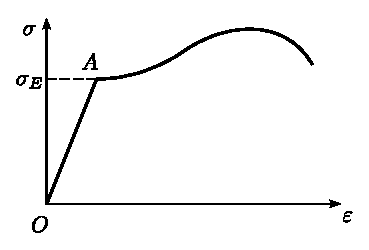
\includegraphics{../images/T1_Ch05-01}
    \end{center}
\end{wrapfigure}
On a vu au \ref{ssec:Ch04-2.1} que le modèle élastique représentait le comportement des matériaux métalliques dans la région élastique, c'est à dire tant que l'on ne dépassait pas le seuil de limite élastique.
Pour justifier les calculs faits avec ce modèle, il faut donc vérifier, après avoir résolu le problème, que ce seuil n'est pas dépassé.Cc'est le principe du calcul élastique des structures ou des éléments de construction.

Dans le cas unidimensionnel, cette vérification se réduit à s'assurer que 
\begin{equation}
    |\sigma| < \sigma_e
    \label{eq:Ch05-057}
\end{equation}
en appelant $\sigma_e$ la limite élastique en traction simple, dont la valeur est également tirée de l'essai de traction. 

Dans le cas tridimensionnel, il faut vérifier un critère de limite d'élasticité qui, de manière générale, peut s'écrire 
\begin{equation}
    f\left( \tens{\sigma} \right) < 0
    \label{eq:Ch05-058}
\end{equation}
où $f$ est une fonction réelle, la fonction seuil élastique, qui limite, dans l'espace des contraintes, la région élastique dans laquelle doit rester le point représentatif des contraintes.

Cette fonction doit vérifier les symétries du matériau, et doit donc être telle que 
\begin{equation}
    f \left( Q_{ik} Q_{il} \sigma_{kl} \right) = f \left( \sigma_{ij} \right)
    \label{eq:Ch05-059}
\end{equation}
pour toute matrice $Q_{ij}$ orthogonale.
En particulier, pour un milieu isotrope, la fonction $f$ doit vérifier l'identité \eqref{eq:Ch05-059} pour toute matrice $Q_{ij}$ orthogonale.
On dit alors que la fonction $f$ est isotrope, et on montre que $f$ est uniquement fonction des invariants principaux de $\tens{\sigma}$, ou ce qui revient au même, fonction symétrique des contraintes principales 
\begin{equation}
    f\left( \tens{\sigma} \right) = f \left( I_1, J_2, J_3 \right) = f\left( \sigma_1, \sigma_2, \sigma_3 \right)
    \label{eq:Ch05-060}
\end{equation}
Plutôt que les invariants $I_1$, $I_2$, $I_3$ de $\tens{\sigma}$ définis par \ref{sec:Ch02-2}, on préfère introduire $I_1$ lié à la partie sphérique de $\tens{\sigma}$ et les invariants $J_2$ du déviateur de $\tens{\sigma}$ \eqref{eq:Ch02-016}.
En effet, ces variables permettent d'obtenir directement la surface seuil dans l'espace des contraintes principales (voir \ref{ssec:Ch02-2.2}).
En particulier, si $J_3$ n'intervient pas dans $f$ alors cette surface seuil est de révolution autour de l'axe hydrostatique.

Pour les métaux, on a montré expérimentalement qu'une pression hydrostatique, aussi élevée soit-elle, ne produisait aucune déformation plastique.
Nous pouvons donc supposer que la partie sphérique du tenseur des contraintes n'intervient pas dans $f$
\begin{equation}
    f \left( J_2, J_3 \right) < 0
    \label{eq:Ch05-061}
\end{equation}
Dans l'espace des contraintes principales, la surface seuil est un cylindre de génératrice parallèle à l'axe hydrostatique.
Le seuil sera donc complètement défini par l'intersection de la surface seuil avec le plan déviatoire (voir \ref{ssec:Ch02-2.2}) ou plutôt, compte tenu des symétries, par cette intersection limitée à un secteur de 60 degrés, le reste étant complété par symétrie.
Il va de soi que la détermination expérimentale de cette courbe est très difficile.
\begin{wrapfigure}{r}{5cm}
    \begin{center}
        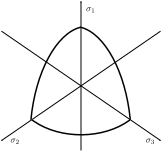
\includegraphics{../images/T1_Ch05-02}
    \end{center}
\end{wrapfigure}

Pour d'autres matériaux, en particulier pour les sols, la «~pression moyenne~» $-\sigma = \frac{1}{3}\sigma_{kk}$ intervient crutialement dans $f$.
On suppose alors souvent que la contrainte principale «~intermédiaire~» n'intervient pas dans $f$ c'est à dire que $f\left( \sigma_1, \sigma_{2}, \sigma_3 \right)$ dépend uniquement de la plus grande et de lit plus petite des contraintes principales.
\begin{equation}
    f = f\left( \sigma_1, \sigma_3 \right) \leq 0 \quad \text{si} \quad \sigma_1 \geq \sigma_2 \geq \sigma_3
    \label{eq:Ch05-062}
\end{equation}
Il ressort alors du paragraphce~\ref{ssec:Ch02-3.1} que, dans la représentation de Mohr, seul intervient le plus grand des trois demi-cerles.
\begin{wrapfigure}{l}{7cm}
    \begin{center}
        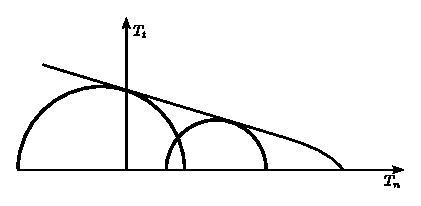
\includegraphics{../images/T1_Ch05-03}
    \end{center}
\end{wrapfigure}
Le critère est alors complètement défini par la «~courbe intrinsèque~» $\mathcal{C}$, enveloppe des demi-cercles limites, c'est à dire à  correspondant à $f=0$. 
C'est le critère de la courbe intrinsèque.

\subsection{Critères de Von Mises et Tresca} \label{ssec:Ch05-3.2}
Pour les métaux, ou plus généralement pour les matériaux dont le critère peut s'écrire sous la forme \eqref{eq:Ch05-061}, on 'utilise habituellement les critères de limite d'élasticité de von Mises ou de Tresca.
Le critère \eqref{eq:Ch05-061} peut s'écrire sous la forme 
\begin{equation}
    -J_2 < \kappa\left( J_3 \right)
    \label{eq:Ch05-063}
\end{equation}
qui, d'après (\ref{eq:Ch02-029},\ref{eq:Ch02-030}), définit l'équation polaire de la courbe seuil dans le plan déviatoire  $\Pi$.
Le critère le plus simple s'obtient en écrivant que $\kappa$ ne dépend pas de $J_3$, c'est à dire que le cylindre seuil est de révolution.

\subsubsection{Critère de von Mises}
\begin{equation}
    -J_2 = \frac{1}{2} s_{ij} s_{ij} < \kappa
    \label{eq:Ch05-064}
\end{equation}
où $\kappa$ est une constante, caractéristique du matériau, et que l'on peut relier à la limite élastique en traction $\sigma_e$.
En traction simple en effet, le critère \eqref{eq:Ch05-064} donne 
\begin{equation*}
    \frac{1}{2} s_{ij} s_{ij} = \frac{\sigma^2}{3} < \kappa
\end{equation*}
soit, par comparaison avec \eqref{eq:Ch05-057}, $\kappa = \sigma_e^2/3$.
Le critère de von Mises s'écrit donc 
\begin{equation}
    \frac{1}{2} s_{ij} s_{ij} < \frac{\sigma_e^2}{3}
    \label{eq:Ch05-065}
\end{equation}
On peut en donner diverses interprétations physiques.
Par exemple, \eqref{eq:Ch05-049} montre que l'énergie de déformation $w$ se décompose en deux parties, une partie due à la dilatation, et une partie due à la distorsion, c'est à dire à la déformation sans changement de volume.
D'après \eqref{eq:Ch05-049}, le critère de von Mises exprime que «~l'énergie de distorsion~» ne doit pas dépasser un certain seuil 
\begin{equation}
    w_{\mathrm{dist}} = \frac{1}{4\mu} s_{ij} s_{ij} < w_{\mathrm{lim}}
    \label{eq:Ch05-065b}
\end{equation}
\begin{wrapfigure}{l}{5cm}
    \begin{center}
        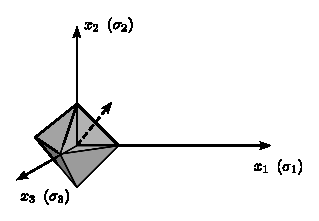
\includegraphics{../images/T1_Ch05-04}
    \end{center}
\end{wrapfigure}
On peut également introduire les «~facettes octaédriques~» normales aux quatre trissectrices des directions principales (ainsi nommées car elles forment un octaèdre).
Les contraintes normale et tangentielle associées à ces facettes sont appelées contraintes normale et tangentielle octaédriques.
En se plaçant en repère principal, un calcul direct montre que 
\begin{equation}
    \begin{aligned}
        T_n^{oct} &= \frac{\sigma_1+\sigma_2+\sigma_3}{3} = \frac{I_1}{3} \\
        T_t^{oct} &= \frac{1}{9}\left\{ \left(\sigma_1-\sigma_2\right)^2 + \left(\sigma_2-\sigma_3\right)^2 + \left(\sigma_3-\sigma_1\right)^2 \right\} = -\frac{2}{3} J_2
    \end{aligned}
    \label{eq:Ch05-066}
\end{equation}
d'après \eqref{eq:Ch02-016}.
Le critère de von Mises exprime donc que la contrainte tangentielle octaédriquene doit pas dépasser un certain seuil 
\begin{equation}
    T_t^{oct} < T_{\mathrm{lim}}
    \label{eq:Ch05-067}
\end{equation}

Le critère de Tresca exprime que la contrainte tangentielle ne doit pas dépasser un certain seuil.

\subsubsection{Critère de Tresca}
\begin{equation}
    T_t = |\vec{T}_t < \kappa
    \label{eq:Ch05-068}
\end{equation}

En un point donné, il faut donc vérifier que le maximum de la contrainte tangentielle, lorsque la facette varie, ne dépasse pas le seuil $\kappa$. 
Compte-tenu des résultats du paragraphe~\ref{ssec:Ch02-3.1}, on peut écrire cette condition 
\begin{equation}
    \mathrm{sup} T_t = \frac{\sigma_1 - \sigma_3}{2} < \kappa \quad \sigma_1 \geq \sigma_2 \geq \sigma_3
    \label{eq:Ch05-069}
\end{equation}
et comme pour le critère de von Mises, on obtient la valeur de $\kappa$ en identifiant \eqref{eq:Ch05-069} à \eqref{eq:Ch05-057} dans le cas de la traction simple.
Il vient 
\begin{equation}
    \sigma_1 - \sigma_3 < \sigma_e \quad \sigma_1 \geq \sigma_2 \geq \sigma_3
    \label{eq:Ch05-070}
\end{equation}
Le critère de Tresca est un critère du type \eqref{eq:Ch05-062}, la courbe intrinsèque étant la droite $T_t = \sigma_e/2$ 
\begin{center}
    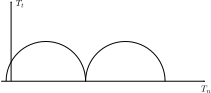
\includegraphics{../images/T1_Ch05-05}
\end{center}

Les deux critères de von Mises et Tresca s'appliquent aux métaux.
Ils conduisent à des résultats légèrement différents.
Par exemple, en cisaillement simple \eqref{eq:Ch02-021}, on obtient comme limite élastique $\tau_2$
\begin{equation}
    \tau_e = 
    \begin{cases}
        \sigma_e /2 & \text{pour Tresca} \\
        \sigma_e /\sqrt{3} & \text{pour von Mises}
    \end{cases}
    \label{eq:Ch05-071}
\end{equation}
Dans l'espace des contraintes principales, la surface seuil est un cylindre à base circulaire pour von Mises, hexagonale pour Tresca 
\begin{center}
    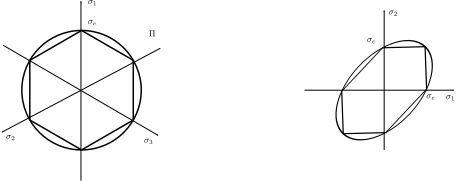
\includegraphics{../images/T1_Ch05-06}
\end{center}
La figure ci-dessus montre l'intersection de ces cylindres avec le plan déviatoire $\Pi$ et avec le plan $\sigma_3=0$, description qui conviendra pour les états de contraintes planes.
Pratiquement, ils conduisent à des résultats suffisamment voisins pour que, dans les applications courantes, on puisse utiliser indifféremment l'un ou l'autre.
On utilisera donc le critère de von Mises lorsque l'on connaîtra le tenseur des contraintes par ses composantes, puisque ce critère s'exprime alors par la relation 
\begin{equation}
    \left( \sigma_{11} - \sigma_{22} \right)^2 + \left( \sigma_{22} - \sigma_{33} \right)^2 + \left( \sigma_{33} - \sigma_{11} \right)^2 + 6\sigma_{12}^2 + 6 \sigma_{23}^2 + 6\sigma_{31}^2 < 2 \sigma_e^2
    \label{eq:Ch05-072}
\end{equation}
Ce critère se prête donc bien aux calculs analytiques ou numériques.
On utilisera le critère de Tresca \eqref{eq:Ch05-070} lorsque l'on connaîtra a priori les directions principales du tenseur des contraintes; il conduira alors à des calculs plus simples que le critère de von Mises. 
